\chapter{The LTLCreator prototype}
\label{chap:theltlcreatorprototype}

As stated in chapter~\ref{chap:goals}, appropriate support by a graphical editor is important for the usefulness of the developed visual language. We therefore designed and implemented a prototype of such an editor which contains the visual language as well as the proposed constraint generation heuristics. The implementation is a java swing component and has a simple API definition, making it easy to integrate the LTLCreator tool into other java applications.

First of all some details about the implementation of the visual language are given in section~\ref{sec:prototype:operatorconstraints}, directly followed by an explanation about the realization of the automated constraint generation functionality in section~\ref{sec:prototype:automatedconstraintgeneration}.
The assembly of all the previous features in one tool is described in section~\ref{sec:coalescence}. However, the tool's functionality shall also be available in Robostudio in order to provide safety mechanisms for the healthcare service robots and to be a prototype for evaluation. Section~\ref{sec:integrationintorobostudio} gives a main idea how an integration into Robostudio ought to be. 



\section{Operator constraints}
\label{sec:prototype:operatorconstraints}

Each of the different operator types, i.e. \emph{IfThenOperator}, \emph{AndOperator}, \emph{OrOperator}, \emph{NotOperator}, \emph{NextOperator}, \emph{FutureOperator}, \emph{AlwaysOperator}, \emph{UntilOperator} and \emph{StateOperator}, has got its own representing class. All of them inherit from one abstract class \emph{AbstractOperator} which provides the basic functionality beeing used by all operators. The \emph{AbstractOperator} class is shown in figure~\ref{fig:abstractoperator} and its methods are described as follows:

\begin{description}
	\item[getLTL():] This function returns the LTL formula of an operator and all its children recursively. Applied to the most outer operator it returns the complete formula for the constraint. This function is abstract and implemented by each operator type separately.
	\item[getColor():] Each operator type has got is own significant color which can be retrieved over the abstract function \emph{getColor()}.
	\item[createNewInstance():] In order to provide operator creation over a tool bar, this function instantiates a new operator object dependet on the implementation.
	\item[setMouseOver(boolean):] Mouse over actions cause the underlying operator to be highlighted. This function makes all operators except the hovered one appearing bleeched out.
	\item[paintOperator(Graphics, ...):] Each operator class has to implement the abstract function \emph{paintOperator()}. It manages all color and shape painting for the respective operator. Additional parameters such as recursive painting including children can be specified.
	\item[contains(int, int):] Given two coordinates x and y, it can be determined wheter the herewith defined point lays within an operator.
	\item[isSimilar(AbstractOperator):] Two operators can be compared for semantic equality. That means same operators with similiar children. This functionality is important for avoiding duplicate constraints during constraint generation.
	\item[addChangeListener(OperatorChangeListener):] Whenever there is a change to the operator or one of its children, an operator change listener gets notified about it. The hierarchical architecture of \emph{AbstractOperator}s propagates all change events to the root operator. The function \emph{addChangeListener()} allows registering for such change notifications.
	\item[removeChangeListener(OperatorChangeListener):] According to \emph{addChangeListener} this function allows deregistration again.
\end{description}

\begin{figure}[htbp]
  \centering
  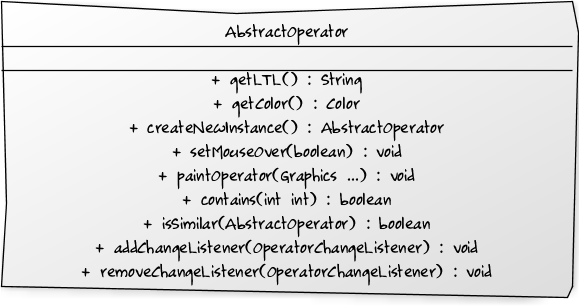
\includegraphics[width=0.6\linewidth]{AbstractOperator} 
  \caption{AbstractOperator class definition.}
  \label{fig:abstractoperator}
\end{figure}

Whereas \emph{StateOperator}s have got no operator children and are leafs in the syntax tree of LTL formulas, all other operator types are either unary or binary operators with respective one or two possible children. 
The graphical representation of both unary and binary operators thus needs to have place holders and docking stations for sub operators. These are realized by buckets which display a small ``drop here'' label and allow operator adding or removing by mouse drops. For this a class Bucket is defined with get and set methods for defining a sub operator.
Figure~\ref{fig:klassendiagramm_operators} depicts the relationship between \emph{AbstractOperator}, \emph{Bucket} and operator implementations.
\begin{figure}[htbp]
  \centering
  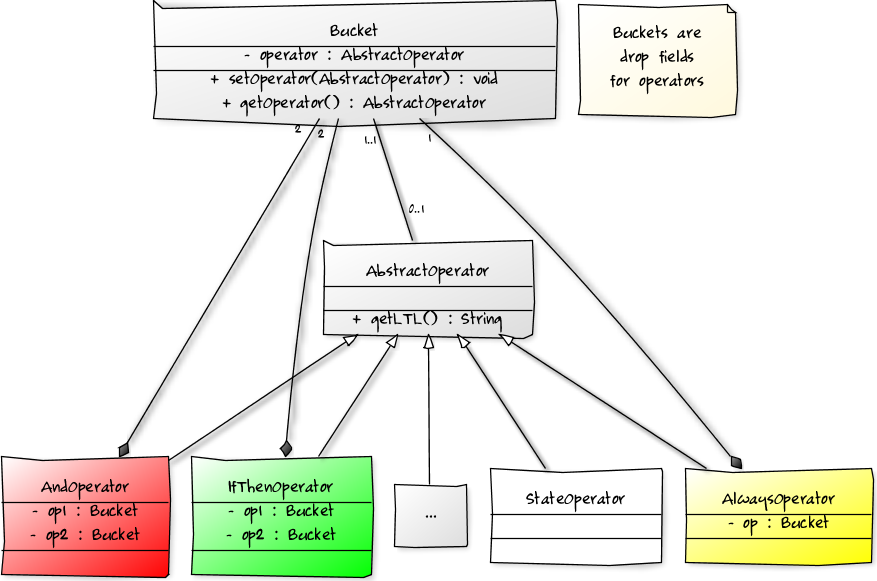
\includegraphics[width=\linewidth]{klassendiagramm_operators} 
  \caption{Class diagram of operator structure.}
  \label{fig:klassendiagramm_operators}
\end{figure}
Once operators are composed in a way that no empty buckets are left over, we retrieve a complete constraint such as the one shown in figure~\ref{fig:operator_tree}. This diagram illustrates the correlation of nested operators and buckets.

\begin{figure}[htbp]
  \centering
  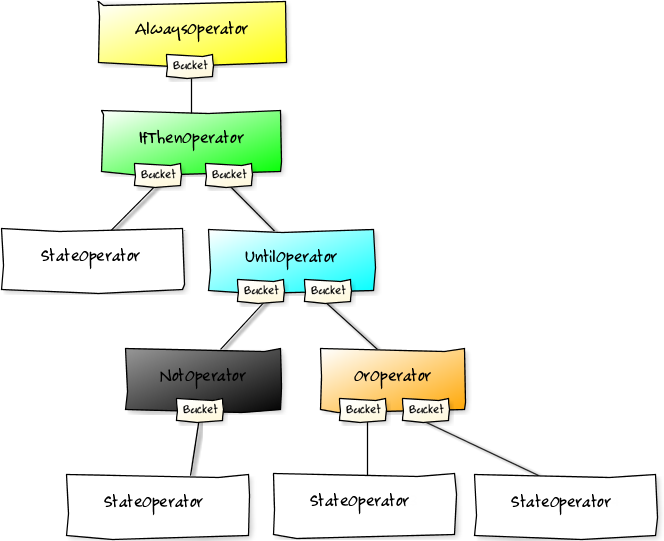
\includegraphics[width=\linewidth]{operator_tree} 
  \caption{Instantiation of a constraint with several operators.}
  \label{fig:operator_tree}
\end{figure}

All graphical components such as buckets and operators are implemented as java swing \emph{JComponent}s. Thereby a lot of functionality for the visual configuration is already available such as the complex layout and repaint concept and the container functionality which is used for unary and binary operators as well as buckets.

%PAINT

For lightweight components swing allows the implementation of a \emph{paint()} method which is responsible for rendering the component. This is used for giving every operator its special look. We hereby made use of swing's \emph{Graphics2D} functionality what gives a great support in painting rounded shapes and color gradients. An operator is displayed as a rounded rectangle with dents around sub operators and has got a flowing backgound, borders and labels in an operator type specific color. For the significant shape multiple rounded rectangles with and without border are arranged in a way that the result appears to be one peace. Figure~\ref{fig:paintprocess} demonstrates how the process of painting is: For painting the if operator first of all a blank rectangle with border is drawn, directly followed by two filled rectangles with border which are placed where later the two child operators shall be. In the third step the same rectangle as from step one just this time without border is painted on top. This makes all crossing borders disappear. Only labels and buckets have to be added yet and a complete \emph{IfThenOperator} emerges.

\begin{figure}[htbp]
  \centering
  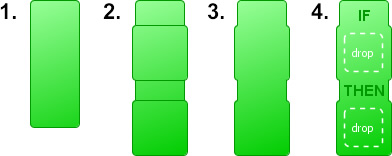
\includegraphics[scale=0.65]{paintprocess} 
  \caption{Four steps of painting an operator.}
  \label{fig:paintprocess}
\end{figure}

%LAYOUT

Swing also provides a mechanism for layouting components, that means depending on child components the aspired sizes and positions of components can be retrieved. As known from figure~\ref{fig:operators} in section~\ref{sec:operatorconstraints} constraints have particular meanings for the two dimensions: a vertical read direction and the horizontal direction for varation in time. This fact forms a special requirement for the layouting of operators.
Whereas the operator's positioning and resizing along the logical direction is only dependend on the sizes of sub operators, the arrangement within the time axis turns out to be more difficult. Here sub operators can't just be aligned centered as it is the case vertically. To face the determination of horizontal positioning, every operator gets time reference lines as depicted in figure~\ref{fig:referencelines}. Logical operators, i.e. \emph{IfThenOperator}, \emph{AndOperator}, \emph{OrOperator}, \emph{NotOperator} and \emph{StateOperator}, have one reference line, time relevant operators, i.e. \emph{NextOperator}, \emph{FutureOperator}, \emph{AlwaysOperator} and \emph{UntilOperator}, have two such reference lines.

\begin{figure}[htbp]
  \centering
  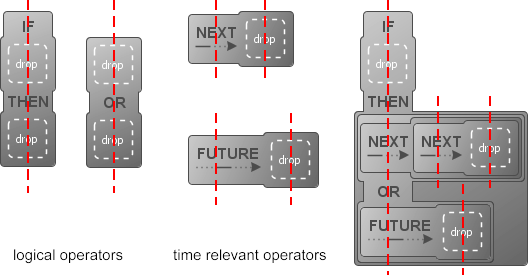
\includegraphics[scale=0.65]{referencelines} 
  \caption{Time reference lines and their adjustments.}
  \label{fig:referencelines}
\end{figure}

%DRAG&DROP

The inbuilt mouse support of swing was used for identifying operators laying under the current mouse position. On the one hand this is important for mouse sensitive highlighting of particular constraint parts, on the other hand this way it can be determined where operators have to be added after drag and drop. So far
% the predefined swing drag and drop has not been used but
a simple drag and drop handler has been implemented.
% instead. 
Once a \emph{JComponent} is registered to the \emph{DndHandler}, it automatically manages any drag and drop actions with \emph{JComponent}s which implement either the \emph{Draggable} or \emph{DropTarget} interface. The former is implemented by all operators, the latter by buckets and the dashboard.
%Figure~\ref{fig:dndclassstructure} gives a short class overview.
Furthermore there is a class \emph{DraggableProvider} which displays a kind of button in the tool bar and lets the user create new \emph{Draggable}s; in our case new operators get instantiated.

\begin{figure}[htbp]
  \centering
  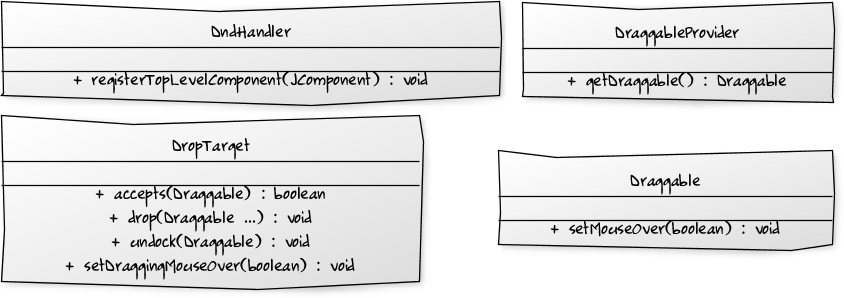
\includegraphics[width=\linewidth]{dndclassstructure} 
  \caption{Class definition for drag and drop functionality.}
  \label{fig:dndclassstructure}
\end{figure}


%operator werden im dashboard, einem weiteren container, zusammengeklickt und angezeigt. Das Dashboard hat dabei eine �hnliche Funktionsweise wie ein Bucket. die operatoren k�nnen dabei vom operatorprovider bezogen werden: Implementierungsdetails? trash...






\section{Automated constraint generation}
\label{sec:prototype:automatedconstraintgeneration}

In section~\ref{chap:automatedconstraintgeneration} we stated that automated constraint generation is based on subgraphs. For the finding of such subgraphs an algorithm has been developed and the main idea how it works is described as follows.

We define one start state and generate all possible paths starting from it leading through the state machine with just one restriction that a path ends before it visits states twice.
Thus we retrieve a finite amount of finite paths since loops are eliminated. Now every state gets a number assigned which represents the total number of occurernces of the respective state in all collected paths. In other words, the label of a state expresses the number of pahts which start in the start state and lead through the respective state. The start state itself has got the number of all paths, of course. If during walking through any of the paths a second state can be found with the same label, it means that all paths starting at start state come all together in this state again. It is uncovered as potential corresponding end state.
A last check has to be applied whether there are incoming transitions from outside into the subgraph which don't come over start state. If no such transitions are detected, a subgraph is found.
If there is no state with the same label, or transitions come from outside, the state machine as a whole can be assumed as subgraph beginning with start state insofar as the state machine doesn't contain further loops or terminating end states. Figure~\ref{fig:subgraph_finding} illustrates this concept of subgraph finding and shows all possible paths as well as the number of occurrence of each state.
This procedure is suitable for bringing to light whether a state is the beginning of a subgraph and for discovering the corresponding end state. In order to detect all subgraphs within a state machine, this procedure has to be applied to every single state.


\begin{figure}[htbp]
  \centering
  
  \tikzstyle{state} = [circle,fill=white,draw]
  \tikzstyle{statein} = [circle,fill=blue!20,draw]
  \tikzstyle{none} = [fill=white]
  \tikzstyle{highlighted} = [fill=yellow]
  \tikzstyle{every path} = [font=\sffamily\small]
  
	\begin{tikzpicture}[->,>=stealth',shorten >=1pt,auto,node distance=15mm]
	
	  \node[state] (1) at (0,0) {A};
	  \node[state] (4) [below left of=1] {B};
	  \node[state] (6) [below of=4] {D};
	  \node[state] (7) [below right of=4] {E};
	  \node[state] (5) [below right of=1] {C};
	  \node[state] (8) [below of=5] {F};
	  \node[state] (9) [below of=7] {G};
	  \node[state] (11) [below left of=9] {H};
	  \node[state] (12) [right of=9] {I};
	  
	  \node[state] (101) at (3,0) {A};
	  \node[state] (102) [below of=101] {B};
	  \node[state] (103) [below of=102] {D};
	  \node[state] (104) [below of=103] {G};
	  \node[state] (105) [below of=104] {H};
	  
	  \node[state] (201) at (4.5,0) {A};
	  \node[state] (202) [below of=201] {B};
	  \node[state] (203) [below of=202] {D};
	  \node[state] (204) [below of=203] {G};
	  \node[state] (205) [below of=204] {I};
	  
	  \node[state] (301) at (6,0) {A};
	  \node[state] (302) [below of=301] {B};
	  \node[state] (303) [below of=302] {E};
	  \node[state] (304) [below of=303] {G};
	  \node[state] (305) [below of=304] {H};
	  
	  \node[state] (401) at (7.5,0) {A};
	  \node[state] (402) [below of=401] {B};
	  \node[state] (403) [below of=402] {E};
	  \node[state] (404) [below of=403] {G};
	  \node[state] (405) [below of=404] {I};
	 
	  \node[state] (501) at (9,0) {A};
	  \node[state] (502) [below of=501] {C};
	  \node[state] (503) [below of=502] {F};
	  \node[state] (504) [below of=503] {G};
	  \node[state] (505) [below of=504] {H};
	  
	  \node[state] (601) at (10.5,0) {A};
	  \node[state] (602) [below of=601] {C};
	  \node[state] (603) [below of=602] {F};
	  \node[state] (604) [below of=603] {G};
	  \node[state] (605) [below of=604] {I};
	 
	  \node[highlighted] (701) at (12,0) {A=6};
	  \node[none] (702) at (12,-0.6) {B=4};
	  \node[none] (703) at (12,-1.2) {C=2};
	  \node[none] (703) at (12,-1.8) {D=2};
	  \node[none] (703) at (12,-2.4) {E=2};
	  \node[none] (703) at (12,-3.0) {F=2};
	  \node[highlighted] (703) at (12,-3.6) {G=6};
	  \node[none] (703) at (12,-4.2) {H=3};
	  \node[none] (703) at (12,-4.8) {I=3};
	  
		%\draw[->] (0, 0) .. controls(1,1) .. (3, 0);
		\draw[->] (12) to [out=45, in=0] (1);
	
	  \path[]
	  	(1) edge node [left] {} (4)
	        edge node [left] {} (5)
	    (4) edge node [left] {} (6)
	        edge node [left] {} (7)
	    (5) edge node [left] {} (8)
	    (6) edge node [left] {} (9)
	    (7) edge node [left] {} (9)
	    (8) edge node [left] {} (9)
	    (11) edge [bend left] node [left] {} (9)
	    (9) edge [bend left] node [left] {} (11)
	    (9) edge node [left] {} (12)
		  
		  
		  (101) edge node [left] {} (102)
		  (102) edge node [left] {} (103)
		  (103) edge node [left] {} (104)
		  (104) edge node [left] {} (105)
		  
		  (201) edge node [left] {} (202)
		  (202) edge node [left] {} (203)
		  (203) edge node [left] {} (204)
		  (204) edge node [left] {} (205)
		  
		  (301) edge node [left] {} (302)
		  (302) edge node [left] {} (303)
		  (303) edge node [left] {} (304)
		  (304) edge node [left] {} (305)
		  
		  (401) edge node [left] {} (402)
		  (402) edge node [left] {} (403)
		  (403) edge node [left] {} (404)
		  (404) edge node [left] {} (405)
		  
		  (501) edge node [left] {} (502)
		  (502) edge node [left] {} (503)
		  (503) edge node [left] {} (504)
		  (504) edge node [left] {} (505)
		  
		  (601) edge node [left] {} (602)
		  (602) edge node [left] {} (603)
		  (603) edge node [left] {} (604)
		  (604) edge node [left] {} (605)
		  ;
	
	\end{tikzpicture}
  \caption{Example for subgraph finding. The occurrence of each state in the paths lets you determine G as an end state corresponding to A.}
  \label{fig:subgraph_finding}
\end{figure}


Following the above description an algorithm has been implemented in java. Its realisation differs from the presented concept in one point that paths are not listed but states are directly labelled since saving all possible paths would be storage inefficient.
The state machine is traversed similarly to a depht-first search and each visited state's label is incremented by one. If the currently visited state holds more than one outgoing transition and thus constitutes new paths,  all states laying on the current stack, i.e. the previously visited states on the current path, get their labels incremented by $(\textnormal{'number of outgoing transitions'} - 1)$. The algorithm turns back whenever it comes across a state which has already been visited within the same path stack of the depth-first search.

The overall implemented way of subgraph finding is illustrated in pseudo code with algorithm~\ref{alg:subgraphfinding}. In line 4 the labelling process described above is executed by using one particular start state. If a state has got the same label as start state has, it is taken as potential end state. Otherwise, the entire state machine is assumed to be a subgraph and start state is taken as end state as well. Subsequent checks finally determine whether it can be considered as proper subgraph.
There are no cycles allowed between start and end state since they're forbidden by the subgraph definition in section~\ref{sec:subgraphdefinition}.
Furthermore also caving transitions are prohibited. Transitions coming from a state outside the subgraph are allowed to lead to the start state but not to other states of the subgraph. If all checks are successful, start and end states get added to the result list $subgraphs$. This proceeding is applied to any state of the state machine what is achieved by a surrounding foreach loop. In the end the list $subgraphs$ contains all pairs of start and end states which form subgraphs.

\begin{algorithm}
\caption{Finding of all subgraphs.}
\label{alg:subgraphfinding}
\begin{algorithmic}[1]
\STATE $subgraphs$: List
\FORALL{states as $S$}
  \STATE $start \leftarrow S$
	\STATE doLabelling($start$);
	\IF{state $E$ exists with label($E$)$=$label($S$)}
		\STATE $end \leftarrow E$
	\ELSE
		\STATE $end \leftarrow start$
	\ENDIF
	\IF{noCycles($start$, $end$) $and$ noExtTransitions($start$, $end$)}
		\STATE $subgraphs$.add($start$, $end$);
	\ENDIF
\ENDFOR
\end{algorithmic}
\end{algorithm}

Depending on size and grade of branch of the state machine, the algorithm for finding subgraphs may take more or less time. To improve user experience during constraint generation a dialog has been implemented which informs the developer about the current progress. This includes the number of found constraints so far and a green bar which gives a percentual estimation of execution time. Furthermore a cancel button permits premature stopping of the execution. A snapshot of the Dialog is shown in figure~\ref{fig:progressdialog}.

\begin{figure}[htbp]
  \centering
  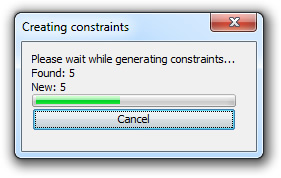
\includegraphics[width=0.40\linewidth]{progressdialog} 
  \caption{Snapshot of the progress dialog displayed during constraint generation.}
  \label{fig:progressdialog}
\end{figure}

The algorithm implementation has been infiltrated by code snippets which frequently interacts with so called \emph{ValidationResultListener}s (figure~\ref{fig:validationresultlistener_class}). This interface is also implemented by the progress dialog. A \emph{ValidationResultListener} has to provide three methods which allow the algorithm to publish the current progress by calling \emph{void setProgress(int)} or to notify about new found subgraphs with invoking \emph{void newSubGraphFound(SubGraph)}. The execution will become terminated whenever \emph{boolean continueGeneration()} returns true.

\begin{figure}[htbp]
  \centering
  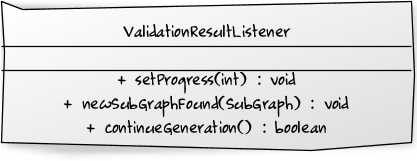
\includegraphics[width=0.55\linewidth]{validationresultlistener_class} 
  \caption{Interface definition of \emph{ValidationResultListener}.}
  \label{fig:validationresultlistener_class}
\end{figure}





\section{Coalescence}
\label{sec:coalescence}

Both features the visual language presented in section~\ref{sec:operatorconstraints} and the automated constraint generation in chapter~\ref{chap:automatedconstraintgeneration} have to be assembled in one tool, the LTLCreator. It shall provide a dashboard with the possibility to manage several constraints, such as a tab panel, and displays for indicating validation results. Besides a button is needed for triggering constraint generation.

Figure~\ref{fig:editor} shows a snapshot of the editor's environment: All functionality needed for constraint editing is provided in the tool bar on the right. It contains draggable elements for creating all operator and proposition types as well as a trashcan for deleting. Constraints can be composed in the dashboard in the center of the editor by drag\&drop which holds and displays the operator constraints. The tab functionality on the left allows multiple constraints to be managed. Each tab shows a small thumbnail of the constraint and a symbol indicating its validity; a warning shield for ``incomplete'', a green shield for ``valid'', a red cross for ``invalid'' or an animated ring for ``validation in progress.''. The magic wand button within the tab pane brings the constraint generation functionality into the editor and triggers the constraint finding process.

\begin{figure}[htbp]
  \centering
  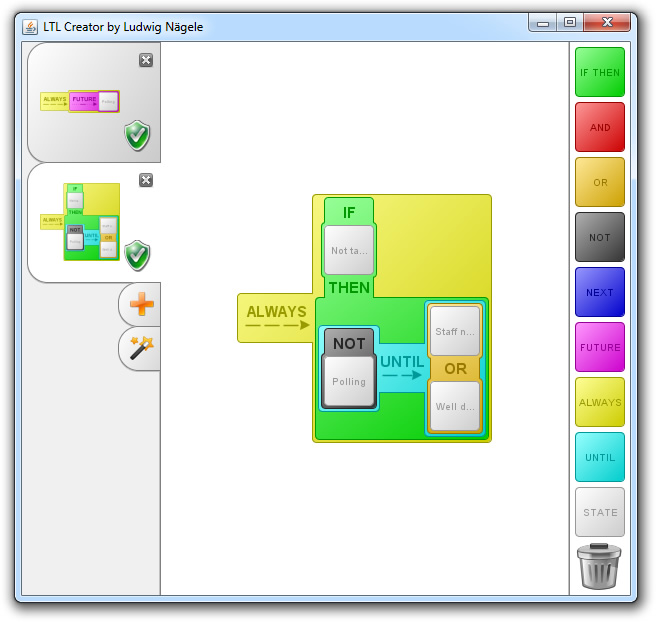
\includegraphics[width=\linewidth]{editor} 
  \caption{Snapshot of the visual editor.}
  \label{fig:editor}
\end{figure}










\subsection{Model checker}

One main requirement of the LTLCreator tool is that all constraints can be validated immediately and allow fast feedback about the correctness of programs. For this a \emph{ConstraintValidator} class has been defined which provides a method \emph{validate(AbstractOperator)} for proving constraints.
For the constraint validation itself a particular model checker can be specified. As a default, the symbolic model checker NuSMV~\cite{springerlink:10.1007/s100090050046,NuSMV2} is used. It is an open source project and has been designed to be an open architecture for model checking. NuSMV doesn't have a java API but it can be externally accessed over command line. For this both the state machine program and the LTL formulas have to be put into file which has to match a NuSMV specific format. An example of this input language is given in listing~\ref{lst:nusmv}.
\singlespacing
\lstset{
  basicstyle=\ttfamily,
  columns=fullflexible,
  showstringspaces=false,
  commentstyle=\color{gray}\upshape
}
\begin{lstlisting}[float = htbp, captionpos=b, breaklines=true, showspaces=false, showtabs=false, tabsize=2, caption=Example of a NuSMV diagram file., label=lst:nusmv]
MODULE main
  VAR
    state: 1..11;
  ASSIGN
    init(state) := 2;
    next(state) := case state = 2 : {3, 1};
                          state = 3 : 1;
                          state = 1 : {2, 4};
                          state = 4 : {1, 5};
                          state = 5 : {6, 9, 10};
                          state = 6 : {7, 8};
                          state = 7 : 8;
                          state = 8 : 1;
                          state = 9 : 11;
                          state = 10 : {9, 11};
                          state = 11 : 1;
                          TRUE : state;
                     esac;

LTLSPEC G (state = 5 -> (F (state = 8 | state = 11)))
\end{lstlisting}
A state machine is encoded in one variable \emph{state}, and its value represents the active state. Thus each state is identified by a number. The state machine described in the example contains eleven states what is determined by the number range for \emph{state} from one to eleven. All variable assignments are specified under \emph{ASSIGN}, what is the semantic equivalent to transition definitions. The initial state can be determined and a case distinction regulates the next possible values, i.e. transitions to reachable states. If there is more than one outgoing transition, all target state identifiers have to be surrounded by brackets. The last expression \emph{TRUE : state;} is a self transition for every state not considered in the case distinction.
The last line contains the constraint formula we want to be checked on the state machine. The prefix \emph{LTLSPEC} just says that NuSMV has to interprete the following constraint as LTL formula.

This kind of output is generated by the \emph{ConstraintValidator} whenever a constraint needs validation. All states are then mapped to numbers and transitions get transormed into case distinctions. The result is stored to file and then loaded by NuSMV. The corresponding valdidation result can be subsequently read from the command line and displayed in the editor next to the visual constraint.

It can happen that there is more than one validation task at a time. This is the case when the constraint generator creates multiple constraints or a change of the state machine causes all constraints to be revalidated at once. Since model checking is a quite ressource inefficient activity, it's recommended to execute all validation tasts consecutively rather than in parallel. A second advantage is that the developer doesn't have to wait for all of them to finish before he can see any result. Since a validation task is not startet until the previous one is finished, constantly new validation results can be displayed to the developer.
All this is managed by the \emph{ValidatorThread}, a queue based mechanism for scheduling validations. Its class definition is presented in figure~\ref{fig:validatorthread_class}.
\begin{figure}[htbp]
  \centering
  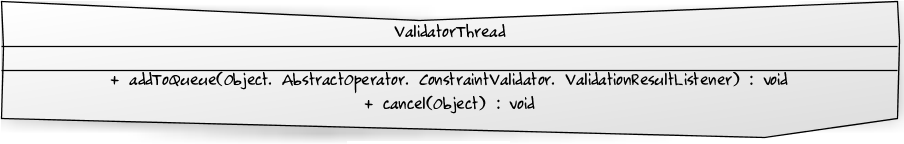
\includegraphics[width=\linewidth]{validatorthread_class} 
  \caption{Class definition of \emph{ValidatorThread}.}
  \label{fig:validatorthread_class}
\end{figure}
Every validation task of a constraint gets enqueued in the \emph{ValidatorThread} after calling the method \emph{addToQueue(...)}.
An identifier is used for each constraint what enables elimination of duplicate tasks for the same constraint in order not to strain the execution time. Tasks can also manually be removed from the queue by calling \emph{cancel(...)}. After a validation task is finished the result is published via callback to the \emph{ValidationResultListener}.









\subsection{Ease of integration}

LTLCreator should be available for other state machine based programming environments for integration what is ensured by its implementation as a java swing component and a clear API enabling the tool for a wide range of use.

Figure~\ref{fig:coalescence} points out how interaction between LTLCreator and programming environments where it is integrated in can be.
\begin{figure}[htbp]
  \centering
  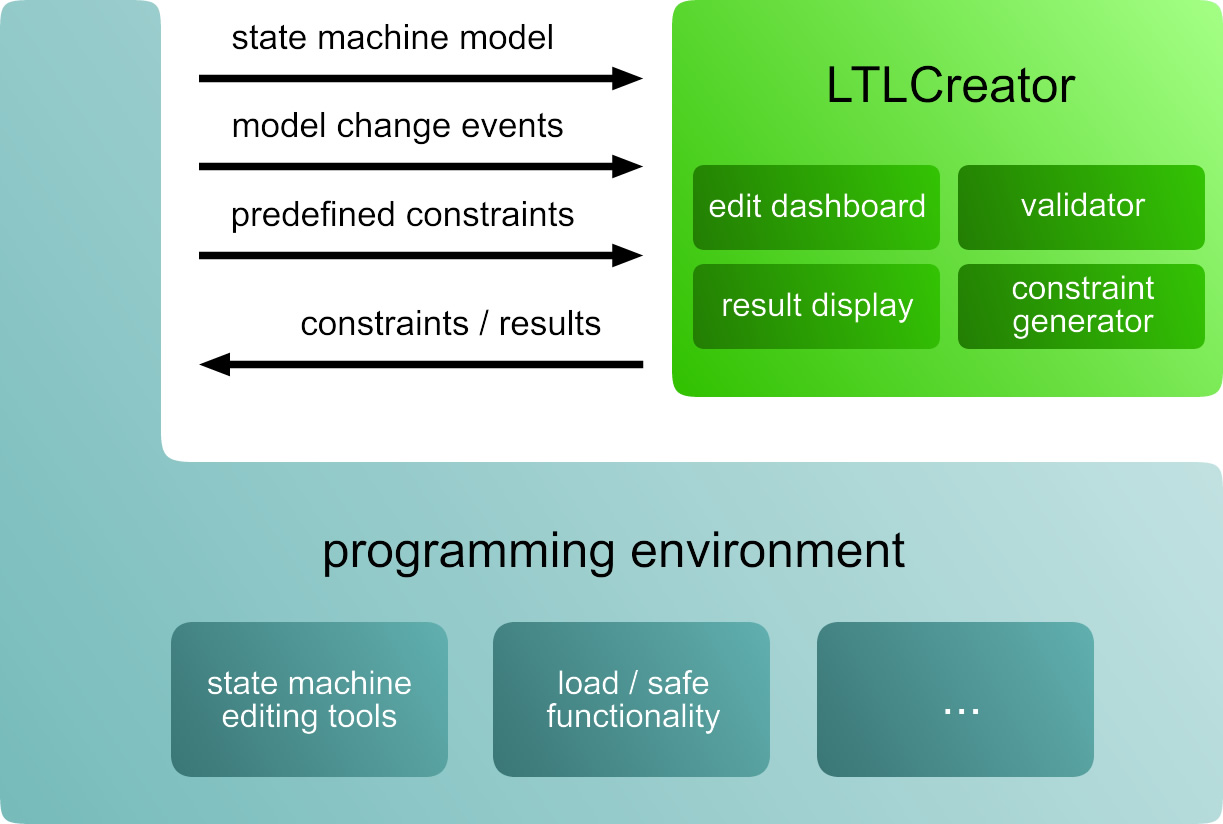
\includegraphics[width=0.7\linewidth]{coalescence}
  \caption{Interaction between LTLCreator and programming environment.}
  \label{fig:coalescence}
\end{figure}
LTLCreator consists of a dashboard where constraints can be edited visually and an graphical output of validation results. The constraint generator as well as the validator are non UI parts of LTLCreator.
The programming environment provides the state machine model and notifies the LTLCreator component about all changes made to the program. This will automatically revalidate all existing constraints and always provide the up-to-date model for constraint generation.
For load and save functionality, all existing constraints can be received and new ones can be added to the LTLCreator component programmatically.
All this functionality can be accessed through methods provided by the component \emph{LTLCreator}. Its class definition is shown in figure~\ref{fig:ltlcreator_class}. Whenever there is a change to the state machine, \emph{setModel(Fsm)} has to be called with the current state machine as parameter. This will cause the editor to revalidate where necessary. Constraint exchange can be done by using the methods \emph{addNewDashboard(AbstractOperator, ...)} and \emph{getOperators()}.

\begin{figure}[htbp]
  \centering
  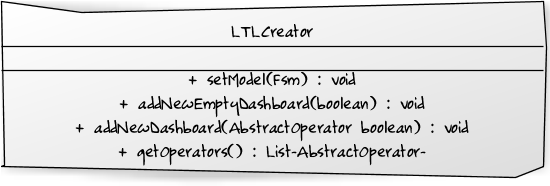
\includegraphics[width=0.65\linewidth]{ltlcreator_class}
  \caption{Class definition of \emph{LTLCreator}.}
  \label{fig:ltlcreator_class}
\end{figure}







\section{Integration into Robostudio}
\label{sec:integrationintorobostudio}

kurz erl�utern, warum das gemaacht werden soll

Robostudio uses NetBeans as a platform, and all tools and features are organized in windows. Thus also LTLCreator has to be put into a window and added to the Robostudio platform. Since the defining of safety constraints is an important part not only after but also during the process of developing service robot behavior, the LTLCreator window as a vital tool shall be placed in the center of the platform where currently also the UI Component Layout Editor Window is. As already proposed in the previous section, all changes to the state machine program made within robostudio must of course cause the LTLCreator window to revalidate all existing constraints.




allein benutzbar, oder ueber robostudio, automatische synchronisierung mit model

%Since Robostudio uses NetBeans as a platform, the LTLCreator has to be integrated as a NetBeans component. Die Datenanbindung zum Austausch des modells (Zustandsmaschine) und der Constraints erfolgt hierbei durch �ffentliche




\subsection{Problems}

(auto-revalidation, model-errors, ...?)
nicht EINE zentrale stelle f�r model�nderungen => zer\-pfl�ck\-te programmierung, wenn man alle �nderungen haben will




\subsection{Solutions}

(pre-checker)

statische analyse